\documentclass[10 pt]{article}
\usepackage{tikz}
\usetikzlibrary{arrows}
\usepackage[margin=0.5 in]{geometry}
\usepackage[utf8]{inputenc}
\usepackage{tabu}
\usepackage{color}
\usepackage{xcolor}
\usepackage{listings}
\usepackage{enumitem}
\usepackage{multicol}
\usepackage[spanish, onelanguage]{algorithm2e}

\setlength{\columnsep}{1cm} 
\title{\textbf {Estructuras de Datos 2 - ST0247\\Segundo Parcial - Jueves (032)}}
\author{Nombre ..............................\\
		Departamento de Informática y Sistemas\\
		Universidad EAFIT\\}
\date{Mayo 09 de 2019}
\begin{document}
\lstdefinestyle{customc}{
	language=Java, 
	numbers=left, 
	showspaces=false,
    showstringspaces=false, 
    tabsize=2, 
    breaklines=true,
    xleftmargin=5.0ex,
}
\lstset{escapechar=@,style=customc, numbers=left, stepnumber = 1} 
\maketitle
\textbf{En las preguntas de selección múltiple, una respuesta incorrecta tendrá
una deducción de 0.2 puntos en la nota final. Si dejas la pregunta sin
responder, la nota será de 0.0. Si no conoces la respuesta, no adivines.}


\begin{multicols}{2}

	\section{Búsqueda Local (20\%)}
	Los algoritmos de ordenamiento son ampliamente usados en diferentes áreas de la Ingeniería de Sistemas como lo es \textit{Big Data}. Debido a esto, es necesario diseñar e implementar algoritmos que resuelvan este problema eficientemente. En este ejercicio, se plantea un algoritmo, que para algunos casos, puede resolver el problema de manera eficiente:
	\begin{algorithm}[H]
		\KwData{Secuencia $a_i$ de $n$ números enteros.}
		\KwResult{Secuencia $a_i'$, tal qué: $a_1' \leq a_2' \leq \cdots \leq a_n'$.}
		$curCost = cost(a)$\;
		\While{$curCost > 0$}{
			\For{$i = 1$ \KwTo $n - 1$}{
				$swap(a_i, a_{i + 1})$\;
				$newCost = cost(a)$\;
				\eIf{$newCost > curCost$}{
					$curCost = newCost$\;	
				}{
					$swap(a_i, a_{i + 1})$\;	
				}
			}
		}
		\caption{Ordenamiento mediante \emph{Búsqueda Local}.}
	\end{algorithm}
	Sabemos que la función $swap(a_i, a_{i+1})$ intercambia los elementos en las posiciones $i$ e $i + 1$ del arreglo $a$. Estamos interesados en encontrar la función de costo $cost(a)$ para la búsqueda. La función de costo simplemente cuenta todos los pares $(a_i, a_j) \mid i < j \land a_j < a_i$. Por favor, completa el siguiente código:
	\begin{lstlisting}
	int cost(int[] a){
	  int respuesta = 0;
	  int n = a.length;
	  for(int i=0; i<n; ++i){
	    for(int j=i+1; j<n; ++j){
	       if(____________){
	          _____________;
	       }
	    }
	  }
	  return respuesta;
	}
	\end{lstlisting}
	\begin{enumerate}[label=\alph*]
		% Respuesta: a[j] < a[i]
		\item (10\%) Completa la línea 6 ................
		% Respuesta: costo += 1
		\item (10\%) Completa la línea 7 ................
	\end{enumerate}


	\section{Programación Dinámica 30\%}
	Hoy, Liko y Kefa encontraron un arreglo de $n$ monedas. En la posición $i$ del arreglo hay --exactamente-- $a_i$ monedas. Ellos quieren saber si pueden repartir las monedas en 2 partes que sumen igual. Ayúdanos, por favor, a resolver este problema. Como un ejemplo, para el arreglo
	$100, 200, 50, 50$ la respuesta es sí porque se puede dar a una persona $100, 50, 50$ y a la otra persona $200$.
	\begin{lstlisting}
	boolean puede(int[] a){
	  int n = a.length;
	  int sum = 0;
	  for(int e: a){
	    sum += e;
	  }
	  if(sum % 2 != 0){
	    ....................;
	  }
	  boolean[][] can = new boolean[sum / 2 + 1][n + 1];
	  for(int i = 0; i <= n; ++i){
	    can[0][i] = true;
	  }
	  for(int i = 1; i <= sum / 2; ++i){
	    can[i][0] = false;
	  }
	  for(int i = 1; i <= sum / 2; ++i){
	    for(int j = 1; j <= n; ++j){
	       can[i][j] = can[i][j - 1];
	       if(i - a[j - 1]>= 0){
		     can[i][j] |= ................;
	       }
	    }
	  }
	  return can[sum / 2][n];
	}
	\end{lstlisting}
	\begin{enumerate}[label=\alph*)]
		\item (10\%) Completa la línea 8  .............
		\item (10\%) Completa la línea 21 .............
		\item (10\%) ¿Cuál es la complejidad asintótica, para el peor de los casos, del algoritmo anterior?
		\begin{enumerate}[label=\roman*)]
			\item $O(n)$
			\item $O(n^2)$
			\item $O(n \times sum)$
			\item $O(n^3)$
		\end{enumerate}
	\end{enumerate}

\section{Dijkstra (30\%)}
	Dado un grafo ponderado y dirigido $G = (V, E, \omega(E))$ y un par de vértices $s, v \in V$, se requiere contar el número de caminos más cortos de $s$ a $v$. Como un ejemplo, para el siguiente grafo, el número de caminos más cortos entre $0$ y $7$ es $3$ ($0-1-4-7$, $0-2-3-5-7$, $0-1-3-5-7$).
		\begin{itemize}[noitemsep]
		
		\item La palabra reservada \textbf{break} termina la ejecución de un ciclo.
		\item La palabra reservada \textbf{continue} interrumpe la ejecución de la iteración actual de un ciclo y empieza una nueva. 
	\end{itemize}
	\begin{center}
		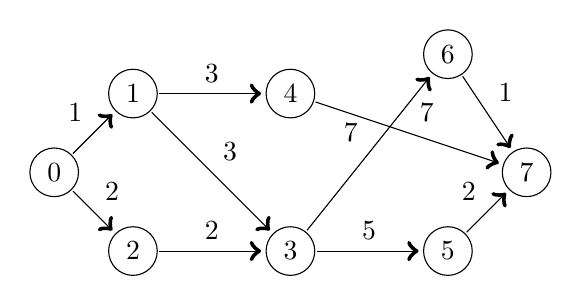
\begin{tikzpicture}	
		\tikzset{shorten >=1pt, auto, node distance=3cm, ultra thick, vertex/.style = {shape=circle,draw,minimum size=1.5em}, edge/.style={draw=black, ultra thick}}
		\tikzset{edge/.style = {-,> = latex'}}
		\node[vertex] (0) at (-1, -1) {0};
		\node[vertex] (1) at (0, 0)  {1};
		\node[vertex] (2) at (0, -2) {2};
		\node[vertex] (3) at (2, -2) {3};
		\node[vertex] (4) at (2, 0) {4};
		\node[vertex] (5) at (4, -2) {5};
		\node[vertex] (6) at (4, 0.5) {6};
		\node[vertex] (7) at (5, -1) {7};
		%edges
		\draw[->] (0) edge node {1} (1);
		\draw[->] (0) edge node {2} (2);
		\draw[->] (1) edge node {3} (3);
		\draw[->] (2) edge node {2} (3);
		\draw[->] (1) edge node {3} (4);
		\draw[->] (4) edge node {7} (7);
		\draw[->] (3) edge node {5} (5);
		\draw[->] (5) edge node {2} (7);
		\draw[->] (3) edge node {7} (6);
		\draw[->] (6) edge node {1} (7);
		\end{tikzpicture}
	\end{center}
	\begin{lstlisting}
	int dijkstra(int[][] g,int s, int v){
	  int n = g.length;
	  int inf = Integer.MAX_VALUE/(2*n);
	  int[] d = new int[n];
	  int[] paths = new int[n];
	  boolean[] w = new boolean[n];
	  Arrays.fill(d, inf);
	  d[s] = 0;
	  paths[s] = ...............;
	  for(int i=0; i<n; i++){
	    int next=-1;
	    for(int j=0; j<n; j++){
	      if(w[j]) continue;
	      if(next==-1 || d[j]<d[next]){
	        next = j;
	      }
	    }
	    if(d[next] == inf) break;
	    w[next] = true;
	    for(int j=0; j<n; j++){
	      int to = j;
	      if(to==next) continue;
	      int weight = g[i][to];
	      int sz = d[next]+weight;
	      if(sz < d[to]){
	        d[to] = sz;
	        paths[to] = ___________;
	      }else if(sz == d[to]){
	        paths[to] = ___________;
	      }
	    }
	  }
	  return paths[v];
	}
	\end{lstlisting}
	\begin{enumerate}[label=\alph*]
		% Respuesta: paths[next]
		\item (10\%) Completa las líneas 8, 27 ................, ...............
		% Respuesta: paths[to] + paths[next]
		\item (10\%) Completa la línea 29 ................
		% Respuesta: O(n^2)
		\item (10\%) Determina la complejidad asintótica, en el peor de los casos, del algoritmo anterior
		\begin{enumerate}[label=\roman*]
			\item $O(n \log n)$
			\item $O(n)$
			\item $O(n^2)$
			\item $O((n \log n) ^ 2)$
		\end{enumerate}
	\end{enumerate}

	\section{Divide y Vencerás 20\%}
	El siguiente algoritmo cálcula $a^b$. Sin embargo, falta algo. Por favor, complétalo.
	\begin{lstlisting}
	int power(int a, int b){
	  if(b == 0) return 1;
	  if(b == 1) return a;
	  int sig = ________________;
	  if(b % 2 != 0) return sig * sig * a;
	  else return sig * sig;
	}
	\end{lstlisting}
	\begin{enumerate}[label=\alph*)]
		\item (10\%) ¿Cuál es la complejidad asintótica, en el peor de los casos, del algoritmo anterior?
		\begin{enumerate}[label=\roman*)]
			\item $O(a)$
			\item $O(b)$
			\item $O(\log(a))$
			\item $O(\log(b))$
		\end{enumerate}
		\item (10\%) Completa la línea 4 ................
	\end{enumerate}
\end{multicols}
\end{document}